
\documentclass[xetex,professionalfont]{beamer}

\usepackage{amsmath}

\usepackage{mathtools}

\usepackage{amssymb}

\usepackage{xspace}

\usepackage{booktabs}


\usepackage{fontspec}
\setmonofont[Scale=0.7]{Droid Sans Mono} %

\usepackage[caption=false]{subfig}
\captionsetup{belowskip=0pt,aboveskip=0pt}

\usepackage{csquotes}

\usepackage{copyrightbox}

\usepackage[english]{babel}


\usepackage{tikz}

\usepackage{pgfplots}

\usetikzlibrary{backgrounds,arrows,automata}

\definecolor{xblue}{RGB}{210,224,255}
\definecolor{xyellow}{RGB}{255,255,205}
\definecolor{xred}{RGB}{255,205,205}
\definecolor{xgreen}{RGB}{205,255,205}


\hypersetup{pdftitle={DLVC Lecture 4},pdfsubject={},pdfauthor={Christopher Pramerdorfer},colorlinks,urlcolor=tuwcvl_cvl_blue,linkcolor=tuwcvl_textlight,citecolor=tuwcvl_textlight}

\makeatletter\renewcommand{\CRB@setcopyrightfont}{\tiny\color{lightgray}}

\let\oldemph\emph
\renewcommand\emph[1]{\textcolor{tuwcvl_cvl_blue}{#1}}

\usefonttheme[onlymath]{serif}

\usetheme{dlvc}


\definecolor{dred}{rgb}{0.85,0,0.1}
\definecolor{dgreen}{rgb}{0,0.85,0.1}
\definecolor{dblue}{rgb}{0,0.1,0.85}


\newcommand{\ie}{\mbox{i.e.}\xspace} %
\newcommand{\eg}{\mbox{e.g.}\xspace} %

\DeclareMathOperator*{\argmin}{arg\,min}
\DeclareMathOperator*{\argmax}{arg\,max}

\newcommand{\NN}{\mathbb{N}}
\newcommand{\ZZ}{\mathbb{Z}}
\newcommand{\QQ}{\mathbb{Q}}
\newcommand{\RR}{\mathbb{R}}

\renewcommand{\vec}[1]{\ensuremath{\mathbf{#1}}}

\newcommand{\va}{\vec{a}}
\newcommand{\vb}{\vec{b}}
\newcommand{\vc}{\vec{c}}
\newcommand{\ve}{\vec{e}}
\newcommand{\vr}{\vec{r}}
\newcommand{\vs}{\vec{s}}
\newcommand{\vt}{\vec{t}}
\newcommand{\vu}{\vec{u}}
\newcommand{\vv}{\vec{v}}
\newcommand{\vw}{\vec{w}}
\newcommand{\vx}{\vec{x}}
\newcommand{\vy}{\vec{y}}
\newcommand{\vz}{\vec{z}}
\newcommand{\vo}{\vec{o}}

\makeatletter
\let\@@magyar@captionfix\relax
\makeatother

\newcommand{\vA}{\vec{A}}
\newcommand{\vW}{\vec{W}}
\newcommand{\vX}{\vec{X}}
\newcommand{\bth}{\boldsymbol{\theta}}
\newcommand{\cD}{\mathcal{D}}

\DeclareMathOperator*{\sgn}{sgn}
\DeclareMathOperator*{\mean}{mean}

\makeatletter
\def\verbatim@font{\linespread{1}\normalfont\ttfamily}
\makeatother


\title{Deep Learning for Visual Computing}
\subtitle{Deep Image Classification}
\author{Christopher Pramerdorfer}
\institute{Computer Vision Lab, TU Wien}

\begin{document}


\begin{frame}
\maketitle
\end{frame}


\begin{frame}
  \frametitle{This Week in AI}
  \framesubtitle{Segment Anything}
  

  \begin{center}
    \copyrightbox[b]
    {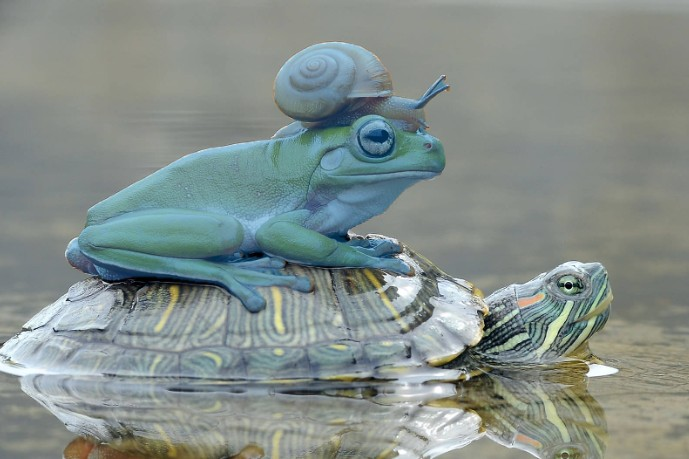
\includegraphics[width=8cm]{images/segment-anything.jpg}}
    {\centering Image from \href{https://segment-anything.com/}{segment-anything}}
  \end{center}
    
\end{frame}


\begin{frame}
\frametitle{Topics}

Deep learning for image classification

\bigskip

Convolutional neural networks
\begin{itemize}
    \item Convolutional layers
    \item Pooling layers
    \item Classification backends
\end{itemize}

\bigskip

Basic classification architectures

\end{frame}


\begin{frame}
\frametitle{Motivation}

At this point we know
\begin{itemize}
    \item That we must tackle large-scale CV problems with ML
    \item How to pose image classification as an ML task
    \item How to extract low-level features from images
    \item What neural networks are and how to train them
\end{itemize}

\bigskip

This is the \emph{traditional image classification pipeline}
\begin{itemize}
    \item Some low-level feature extractor (e.g.~HoG)
    \item Some form of dimensionality reduction (e.g.~PCA)
    \item Some generic classification model (e.g.~MLP)
\end{itemize}

\end{frame}


\begin{frame}
\frametitle{Motivation}

This pipeline performs poorly on large-scale problems
\begin{itemize}
    \item Can only extract indiscriminative low-level features
    \item CIFAR-10 test accuracy only $\approx 60\%$ (HoG + MLP)
\end{itemize}

\bigskip

\begin{center}
    \copyrightbox[b]
    {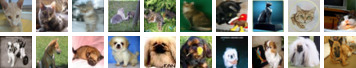
\includegraphics[width=10cm]{images/cifar10-catsdogs.jpg}}
    {\centering Image from cs.toronto.edu}
\end{center}

\end{frame}


\begin{frame}
\frametitle{Motivation}

We cannot design reliable high-level feature extractors

\bigskip

But we can try to learn them
\begin{itemize}
    \item Approach is called \emph{representation learning}
\end{itemize}

\bigskip

In theory we can do so using MLPs %
\begin{itemize}
    \item Use image vectors as inputs
    \item Hidden layer(s) extract features
    \item Output layer acts as linear classifier
\end{itemize}

\end{frame}


\begin{frame}
\frametitle{Motivation}

This usually does not work well though %
\begin{itemize}
    \item $\dim(\bth)$ increases quickly with image size \& model capacity
    \item MLPs are designed for arbitrary vector inputs, not images
    \item Complex MLPs are hard to train %
\end{itemize}

\smallskip

\begin{center}
\begin{tikzpicture}[every node/.style={scale=0.75}]
    \node[anchor=south west,inner sep=0] (image) at (0,0) {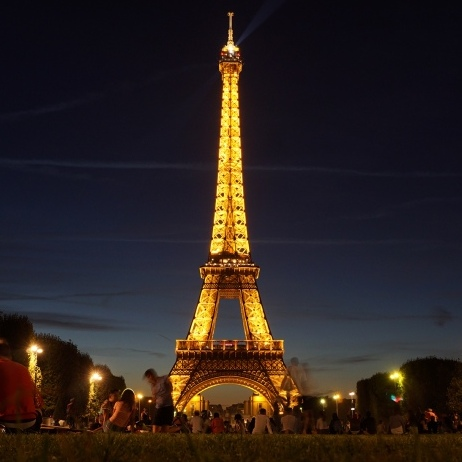
\includegraphics[width=4.5cm]{images/eiffel-tower.jpg}};
    \begin{scope}[x={(image.south east)},y={(image.north west)}]
        \draw[step=0.02, dblue] (0,0) grid (0.998,1.022);
        \foreach \x in {0.01,0.05,...,1} {
            \foreach \y in {0.01,0.05,...,1.02} {
                \draw[gray,opacity=0.33] (\x,\y) -- (1.3, 0.5);
            }
        }
        \foreach \x in {0.1,0.2,...,0.8} {
            \draw[dred,thick,fill=white] (1.3,\x) circle (0.05cm);
        }
        \node at (1.3,0.95) {$\vdots$};
        \node at (1.3,0) {$\vdots$};
    \end{scope}
\end{tikzpicture}
\end{center}

\end{frame}


\begin{frame}
\frametitle{Motivation}

We clearly need a better neural network architecture
\begin{itemize}
    \item Optimized for image data
    \item Fewer parameters per layer (easier to increase depth) %
\end{itemize}

\bigskip

Let us derive such an architecture from MLPs
\begin{itemize}
    \item By introducing reasonable \emph{inductive biases}
    \item Assumptions built into the model or training pipeline
    \item To improve model performance and/or efficiency
\end{itemize}

\end{frame}


{
\setbeamertemplate{footline}{}
\begin{frame}

\begin{tikzpicture}[remember picture,overlay]
\fill[white] (current page.north west) rectangle (current page.south east);
\end{tikzpicture}

\begin{center}
\textcolor[rgb]{0.9,0.9,0.9}{blank page}
\end{center}

\end{frame}
}


\begin{frame}
\frametitle{Convolutional Neural Networks}
\framesubtitle{Input Layer}

Network should make use of spatial structure of images
\begin{itemize}
    \item Not sensible to flatten images to vectors
\end{itemize}

\bigskip

We represent them as 3D tensors $\vX$ instead
\begin{itemize}
    \item \emph{Tensors} are $n$-dimensional generalizations of matrices
\end{itemize}

\bigskip

We will use $C\times H\times W$ dimension order
\begin{itemize}
    \item Same order as PyTorch
    \item $3\times32\times32$ for CIFAR-10
\end{itemize}

\end{frame}


\begin{frame}
\frametitle{Convolutional Neural Networks}
\framesubtitle{Input Layer}

Input neurons form $C_0\times H_0\times W_0$ grid

\begin{center}
\begin{tikzpicture}
    \node (image) at (-5,0) {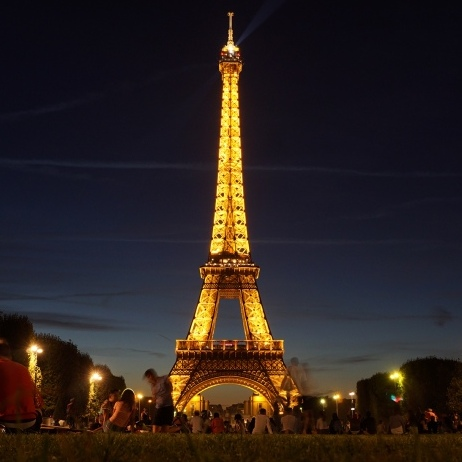
\includegraphics[width=4cm]{images/eiffel-tower.jpg}};
    \node (image3) at (0.4,0.4) {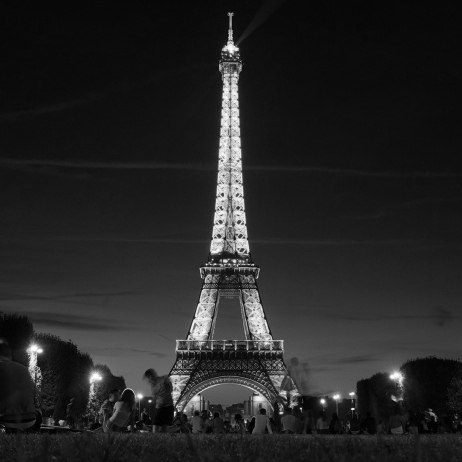
\includegraphics[width=3.92cm]{images/eiffel-tower-gray.jpg}};
    \draw[step=0.08, dblue, opacity=0.5] (-1.55 cm, -1.55 cm) grid (2.35 cm,2.35 cm);
    \node (image3) at (0.2,0.2) {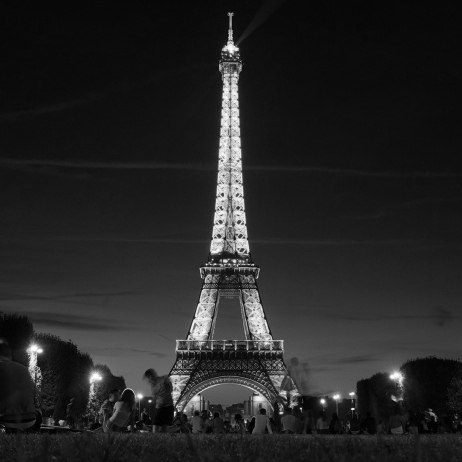
\includegraphics[width=3.92cm]{images/eiffel-tower-gray.jpg}};
    \draw[step=0.08, dgreen, opacity=0.5] (-1.75 cm, -1.75 cm) grid (2.15 cm,2.15 cm);
    \node (image3) at (0,0) {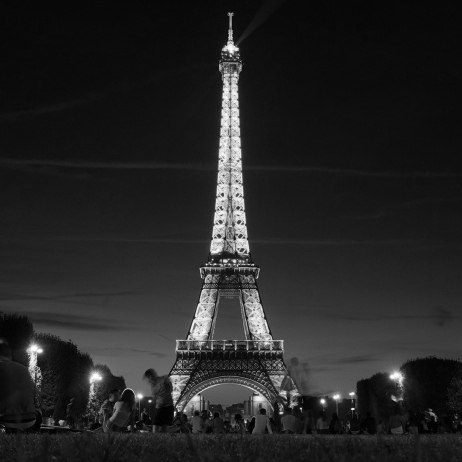
\includegraphics[width=3.92cm]{images/eiffel-tower-gray.jpg}};
    \draw[step=0.08, dred, opacity=0.5] (-1.95 cm, -1.95 cm) grid (1.95 cm,1.95 cm);
    \node at (-5,-2.5 cm) {\small Input Image};
    \node at (0,-2.5 cm) {\small Input Layer};
\end{tikzpicture}
\end{center}

\end{frame}


\begin{frame}
\frametitle{Convolutional Neural Networks}
\framesubtitle{Feature Extraction}

Spatially close pixels are highly correlated, others are not
\begin{itemize}
    \item Nearby pixels likely correspond to same object (part)
\end{itemize}

\bigskip

A good image feature extraction layer should account for this
\begin{itemize}
    \item Compute \emph{local features} from spatially close inputs %
\end{itemize}

\bigskip

We can achieve this by
\begin{itemize}
    \item Arranging hidden layer neurons in $W_l\times H_l$ grid
    \item Connecting only spatially close neurons %
    \item Neurons are thus \emph{sparsely connected} (fewer parameters)
\end{itemize}

\end{frame}


\begin{frame}
\frametitle{Convolutional Neural Networks}
\framesubtitle{Feature Extraction}

\begin{center}
    \copyrightbox[b]
    {
    \begin{tikzpicture}
    \node (image) at (0,0) {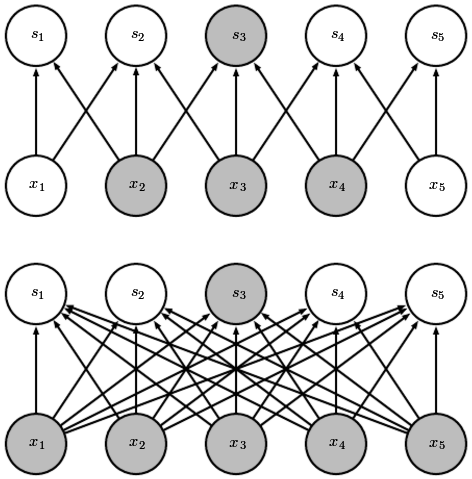
\includegraphics[width=5cm]{images/connectivity}};
    \node[right] at (2.5 cm, 1.3 cm) {\small Sparse Connectivity}; %
    \node[right] at (2.5 cm, -1.4 cm) {\small Dense Connectivity (MLP)}; %
    \end{tikzpicture}
    }
    {\centering Image adapted from [1]}
\end{center}

\end{frame}


\begin{frame}
\frametitle{Convolutional Neural Networks}
\framesubtitle{Feature Extraction}

$W_l$ and $H_l$ depend on input width and height %
\begin{itemize}
    \item Usually $W_l=W_{l-1}$ and $H_l=H_{l-1}$ to preserve resolution
    \item Padding in border regions (replication) %
\end{itemize}

\bigskip

Connectivity $k$ along $W$ and $H$ dimensions
\begin{itemize}
    \item Configurable but often $k=3$, that is $3\times3$
\end{itemize}

\bigskip

Connectivity along channel dimension is usually $C_{l-1}$ %
\begin{itemize}
    \item Want to make use of all local information
\end{itemize}

\end{frame}


\begin{frame}
\frametitle{Convolutional Neural Networks}
\framesubtitle{Feature Extraction}

\begin{center}
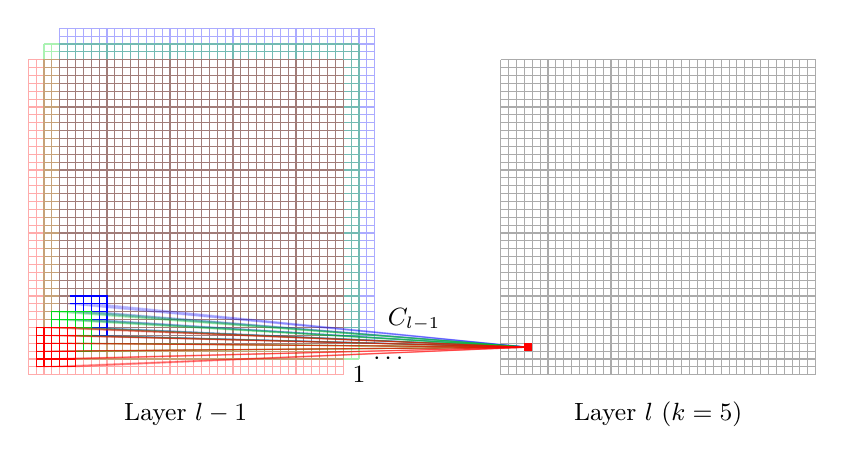
\begin{tikzpicture}
\draw[step=0.1, blue, opacity=0.33] (0.4,0.4) grid (4.401,4.401);
\draw[step=0.1, dgreen, opacity=0.33] (0.2,0.2) grid (4.201,4.201);
\draw[step=0.1, red, opacity=0.33] (0.0,0.0) grid (4.001,4.001);
\node at (2,-0.5) {\small Layer $l-1$};
\node at (4.2,0.0) {\small $1$};
\node at (4.6,0.2) {\small $\cdots$};
\node at (4.9,0.7) {\small $C_{l-1}$};
\draw[step=0.1, black, opacity=0.33] (6.0,0.0) grid (10.001,4.001);
\node at (8,-0.5) {\small Layer $l$ ($k=5$)};
\draw[step=0.1, blue] (0.53,0.5) grid (1.01,1.01);
\foreach \x in {0.5,0.6,...,1.0} {
    \foreach \y in {0.5,0.6,...,1.0} {
        \draw[blue,opacity=0.2] (\x,\y) -- (6.35, 0.35);
    }
}
\draw[step=0.1, dgreen] (0.3,0.3) grid (0.81,0.81);
\foreach \x in {0.3,0.4,...,0.8} {
    \foreach \y in {0.3,0.4,...,0.8} {
        \draw[dgreen,opacity=0.2] (\x,\y) -- (6.35, 0.35);
    }
}
\draw[step=0.1, red] (0.1,0.1) grid (0.61,0.61);
\foreach \x in {0.1,0.2,...,0.6} {
    \foreach \y in {0.1,0.2,...,0.6} {
        \draw[red,opacity=0.2] (\x,\y) -- (6.35, 0.35);
    }
}
\draw[draw=none,fill=red] (6.3, 0.3) rectangle (6.4, 0.4);
\end{tikzpicture}
\end{center}

\end{frame}


\begin{frame}
\frametitle{Convolutional Neural Networks}
\framesubtitle{Feature Extraction}

Extraction should work the same anywhere in input %
\begin{itemize}
    \item We generally don't know where objects will appear
    \item Due to varying object location and viewpoint %
\end{itemize}

\bigskip

Achieved by letting neurons compute the same operation
\begin{itemize}
    \item For linear layers this means identical weights and bias
    \item So $o_h=\vW_l\cdot\vX_h+b_l$ with $\vX_h,\vW_l\in\RR^{C_{l-1}\times k\times k}$ %
\end{itemize}

\end{frame}


\begin{frame}
\frametitle{Convolutional Neural Networks}
\framesubtitle{Feature Extraction}

Neurons in layer $l$ compute $o_h=\vW_l\cdot\vX_h+b_l$
\begin{itemize}
    \item $\vW_l\cdot\vX_h$ is a linear combination (like before)
    \item $\vW_l$ is identical for all neurons in layer
\end{itemize}

\bigskip

The overall transformation of the layer is thus
\begin{itemize}
     \item A \emph{convolution} of the input with kernel $\vW_l$
     \item Followed by an additive bias $b_l$
\end{itemize}

\bigskip

Such layers are thus called \emph{convolutional layers}
\begin{itemize}
    \item Or \emph{conv layers} for short
\end{itemize}

\end{frame}


\begin{frame}
\frametitle{Convolutional Neural Networks}
\framesubtitle{Feature Extraction}

Recall how discrete convolutions work (here $C_{l-1}=1$)

\medskip

\begin{center}
    \copyrightbox[b]
    {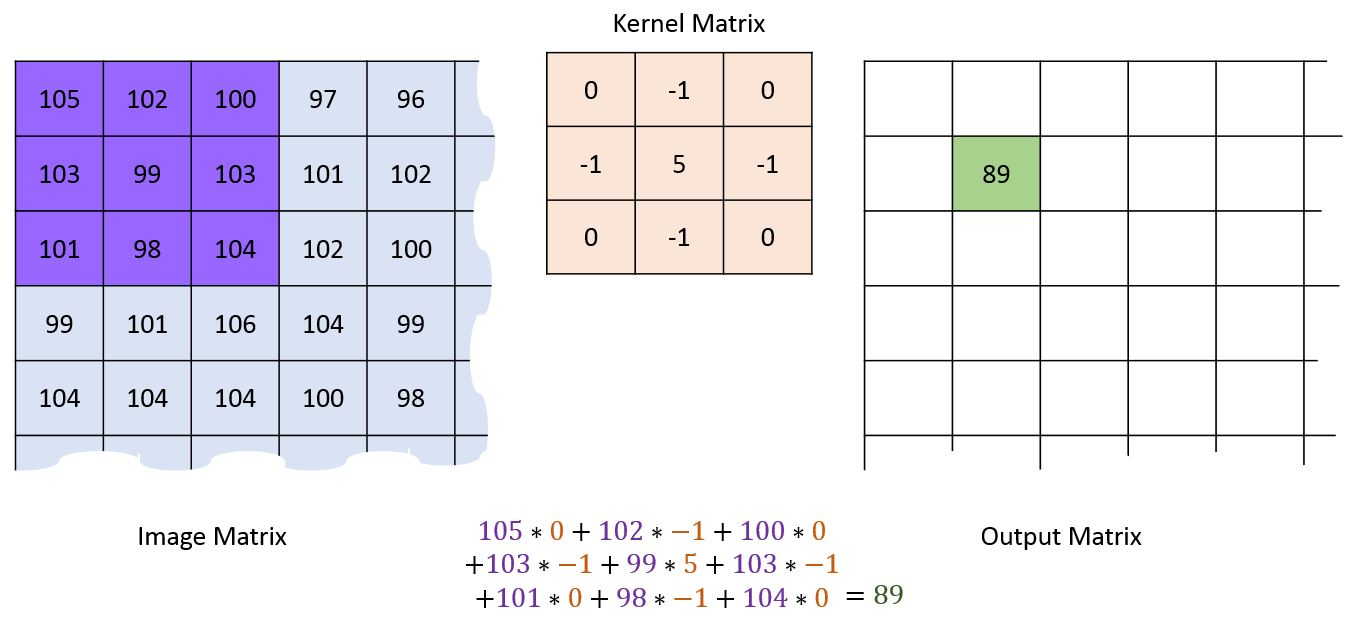
\includegraphics[width=10cm]{images/conv2d}}
    {\centering Image from \href{http://machinelearninguru.com/computer_vision/basics/convolution/image_convolution_1.html}{machinelearninguru.com}}
\end{center}

\end{frame}


\begin{frame}
\frametitle{Convolutional Neural Networks}
\framesubtitle{Feature Extraction}

Recall how discrete convolutions work (here $C_{l-1}=1$)

\medskip

\begin{center}
    \copyrightbox[b]
    {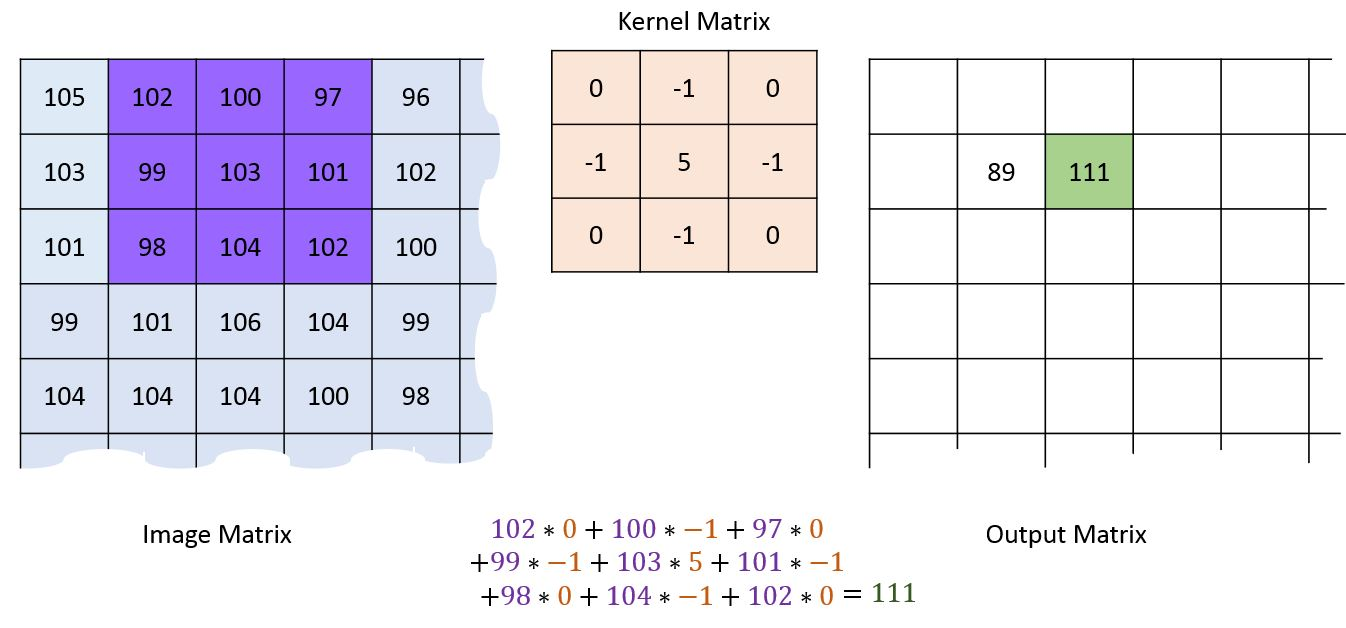
\includegraphics[width=10cm]{images/conv2d-2}}
    {\centering Image from \href{http://machinelearninguru.com/computer_vision/basics/convolution/image_convolution_1.html}{machinelearninguru.com}}
\end{center}

\end{frame}


\begin{frame}
\frametitle{Convolutional Neural Networks}
\framesubtitle{Feature Extraction}

Neurons thus \enquote{detect} features via $o_h=\vW_l\cdot\vX_h+b_l$
\begin{itemize}
    \item Respond to local structures similar to $\vW_l$
    \item Similar to template matching with \emph{learned template} $\vW_l$
\end{itemize}

\bigskip

Conv layers are thus rather simple feature extractors
\begin{itemize}
    \item Power comes from stacking such layers %
    \item With activation functions (ReLU) and other layers in between
\end{itemize}

\end{frame}


\begin{frame}
\frametitle{Convolutional Neural Networks}
\framesubtitle{Feature Extraction}

One issue remains
\begin{itemize}
    \item Every neuron performs same operation
    \item So layer can learn to extract only one feature
\end{itemize}

\bigskip

To overcome this problem we replicate the neurons $C_l$ times
\begin{itemize}
    \item Resulting in a $C_l\times W_l\times H_l$ grid of neurons
    \item Arranged in $C_l$ \emph{feature maps} of size $W_l\times H_l$
\end{itemize}

\bigskip

Layer can thus learn $C_l$ different features
\begin{itemize}
    \item Only neurons in same feature map (channel) share parameters
\end{itemize}

\end{frame}


\begin{frame}
\frametitle{Convolutional Neural Networks}
\framesubtitle{Feature Extraction}

\begin{center}
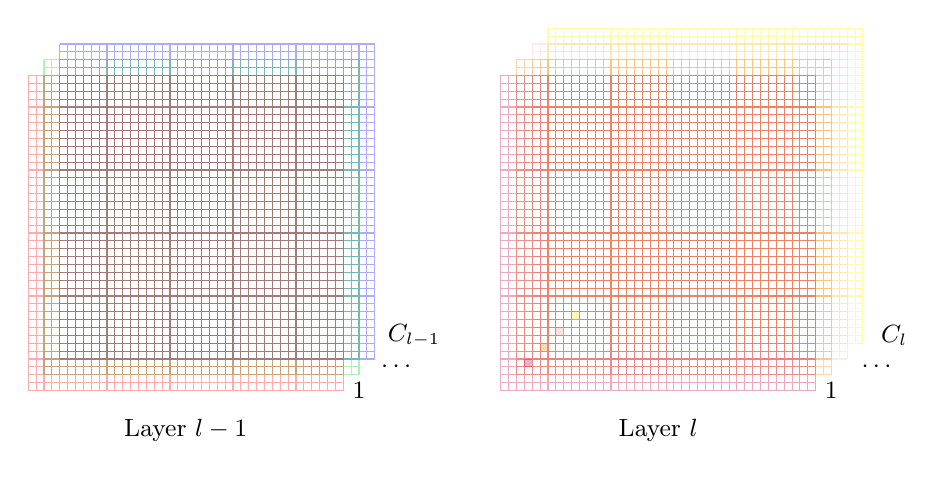
\begin{tikzpicture}
\draw[step=0.1, blue, opacity=0.33] (0.4,0.4) grid (4.401,4.401);
\draw[step=0.1, dgreen, opacity=0.33] (0.2,0.2) grid (4.201,4.201);
\draw[step=0.1, red, opacity=0.33] (0.0,0.0) grid (4.001,4.001);
\node at (2,-0.5) {\small Layer $l-1$};
\node at (4.2,0.0) {\small $1$};
\node at (4.7,0.3) {\small $\cdots$};
\node at (4.9,0.7) {\small $C_{l-1}$};
\draw[step=0.1, yellow, opacity=0.33] (6.6,0.6) grid (10.601,4.601);
\draw[step=0.1, pink, opacity=0.33] (6.4,0.4) grid (10.401,4.401);
\draw[step=0.1, orange, opacity=0.33] (6.2,0.2) grid (10.201,4.201);
\draw[step=0.1, purple, opacity=0.33] (6.0,0.0) grid (10.001,4.001);
\node at (8,-0.5) {\small Layer $l$};
\node at (10.2,0.0) {\small $1$};
\node at (10.8,0.3) {\small $\cdots$};
\node at (11.0,0.7) {\small $C_l$};
\draw[draw=none,fill=yellow, opacity=0.3] (6.9, 0.9) rectangle (7.0, 1.0);
\draw[draw=none,fill=pink, opacity=0.5] (6.7, 0.7) rectangle (6.8, 0.8);
\draw[draw=none,fill=orange, opacity=0.3] (6.5, 0.5) rectangle (6.6, 0.6);
\draw[draw=none,fill=purple, opacity=0.3] (6.3, 0.3) rectangle (6.4, 0.4);
\end{tikzpicture}
\end{center}

\end{frame}


\begin{frame}
\frametitle{Convolutional Neural Networks}
\framesubtitle{Feature Extraction}

Number of weights $\vW_l$ depends only on $k,\,C_{l-1},\,C_l$ %
\begin{itemize}
    \item $k=3,\,C_{l-1}=3,\,C_l=32\implies864$ weights %
    \item $k=3,\,C_{l-1}=32,\,C_l=64\implies18.5$k weights %
\end{itemize}

\bigskip

Way fewer parameters than with linear layers
\begin{itemize}
    \item Can stack many conv layers
    \item Layer $l$ learns to combine layer $l-1$ features to new ones
\end{itemize}

\end{frame}


\begin{frame}
\frametitle{Convolutional Neural Networks}
\framesubtitle{Feature Extraction}

Neurons see only small part of previous layer (sparse connectivity) %
\begin{itemize}
    \item But larger input region (\emph{receptive field}) as depth increases %
\end{itemize}

\

\begin{center}
    \copyrightbox[b]
    {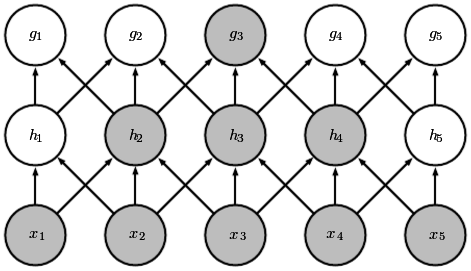
\includegraphics[width=5.5cm]{images/receptive-field}}
    {\centering Image from [1]}
\end{center}

\end{frame}


\begin{frame}
\frametitle{Convolutional Neural Networks}
\framesubtitle{Feature Extraction}

So in networks of conv layers
\begin{itemize}
    \item Direct connections are sparse
    \item But receptive field can span most/all of image %
\end{itemize}

\bigskip

Feature extraction approach is thus part-based %
\begin{itemize}
    \item Learn local features (e.g. presence of eye or nose)
    \item Learn more global features (e.g. presence of face) from those
\end{itemize}

\bigskip

Hierarhical approach to representation learning
\begin{itemize}
    \item Divide and conquer
\end{itemize}

\end{frame}


\begin{frame}
\frametitle{Convolutional Neural Networks}
\framesubtitle{Feature Extraction}

\begin{center}
\copyrightbox[b]
{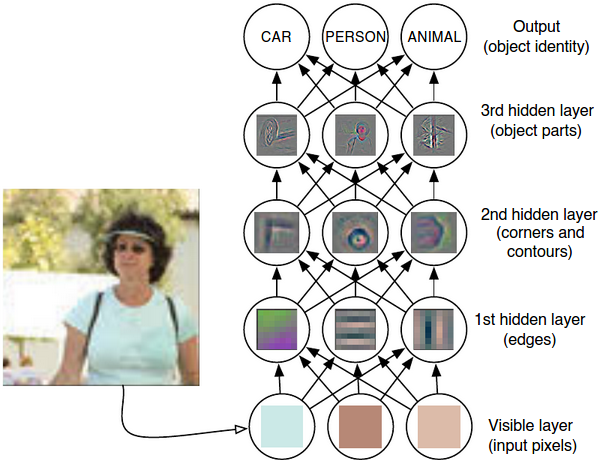
\includegraphics[width=7cm]{images/dl-layer-example}}
{\centering Image from [1]}
\end{center}

\end{frame}


\begin{frame}
\frametitle{Convolutional Neural Networks}
\framesubtitle{Feature Extraction}

Conv layers are fundamental deep learning layers
\begin{itemize}
    \item Part of most network architectures for image analysis %
\end{itemize}

\bigskip

Networks with conv layers are \emph{convolutional neural networks}
\begin{itemize}
    \item \emph{CNNs} or \emph{convnets} for short
\end{itemize}

\end{frame}


\begin{frame}
\frametitle{Convolutional Neural Networks}
\framesubtitle{Pooling}

Recall that conv layers
\begin{itemize}
    \item Retain the input size $W_{l-1}\times H_{l-1}$ (padding)
    \item Or reduce it only slowly (no padding) %
\end{itemize}

\bigskip

This
\begin{itemize}
    \item Slows down computations %
    \item Leads to shallow receptive fields %
\end{itemize}

\bigskip

We thus want some form of \emph{pooling} %
\begin{itemize}
    \item Reduce $W_{l-1}$ and $H_{l-1}$ via local aggregation %
\end{itemize}

\end{frame}


\begin{frame}
\frametitle{Convolutional Neural Networks}
\framesubtitle{Pooling}

\emph{Pooling layers} are an example
\begin{itemize}
    \item Process input channels independently %
    \item Aggregate via $\max(\vX_h)$ or $\mean(\vX_h)$
    \item Leave $C_{l-1}$ unchanged
\end{itemize}

\end{frame}


\begin{frame}
\frametitle{Convolutional Neural Networks}
\framesubtitle{Pooling}

$2\times2$ \emph{max-pooling} layer with \emph{stride} $2$
\begin{itemize}
    \item $W_l=W_{l-1}/2$, $H_l=H_{l-1}/2$, and $k=2$
    \item Output of neuron $h$ is $\max(\vX_h)$ with $\vX_h\in\RR^{2\times2}$
\end{itemize}

\smallskip

\begin{center}
    \copyrightbox[b]
    {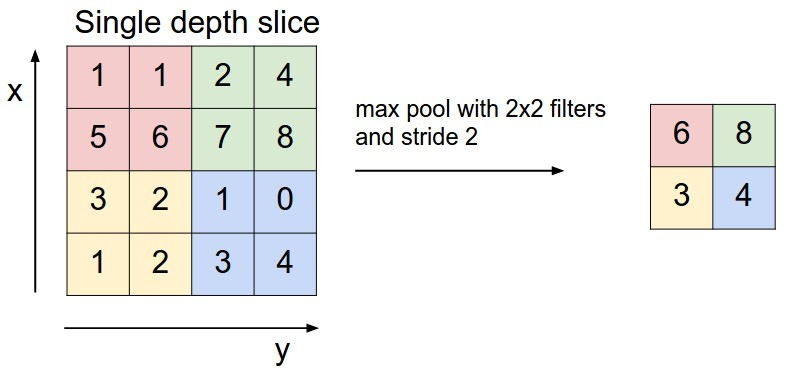
\includegraphics[width=7cm]{images/maxpool}}
    {\centering Image from \href{https://cs231n.github.io/convolutional-networks/}{cs231n.github.io}}
\end{center}

\end{frame}


\begin{frame}
\frametitle{Convolutional Neural Networks}
\framesubtitle{Pooling}

Number of neurons reduced by factor $4$  %
\begin{itemize}
    \item Corresponding efficiency increase
    \item At the cost of losing spatial resolution %
\end{itemize}

\bigskip

\begin{center}
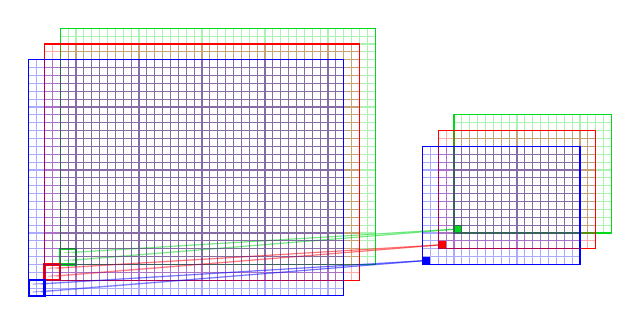
\begin{tikzpicture}
\draw[step=1mm,dgreen,opacity=0.33] (0.4,0.4) grid (4.4,3.4);
\draw[dgreen] (0.4,0.4) rectangle (4.4,3.4);
\draw[step=1mm,dgreen,opacity=0.33] (5.4,0.8) grid (7.4,2.3);
\draw[dgreen] (5.4,0.8) rectangle (7.4,2.3);
\draw[dgreen,thick] (0.4,0.4) rectangle (0.6,0.6);
\draw[draw=none,fill=dgreen] (5.4,0.8) rectangle (5.5,0.9);
\draw[dgreen,opacity=0.33] (0.45,0.45) -- (5.45, 0.85);
\draw[dgreen,opacity=0.33] (0.55,0.45) -- (5.45, 0.85);
\draw[dgreen,opacity=0.33] (0.45,0.55) -- (5.45, 0.85);
\draw[dgreen,opacity=0.33] (0.55,0.55) -- (5.45, 0.85);
\draw[step=1mm,red,opacity=0.33] (0.2,0.2) grid (4.2,3.2);
\draw[red] (0.2,0.2) rectangle (4.2,3.2);
\draw[step=1mm,red,opacity=0.33] (5.2,0.6) grid (7.2,2.1);
\draw[red] (5.2,0.6) rectangle (7.2,2.1);
\draw[red,thick] (0.2,0.2) rectangle (0.4,0.4);
\draw[draw=none,fill=red] (5.2,0.6) rectangle (5.3,0.7);
\draw[red,opacity=0.33] (0.25,0.25) -- (5.25, 0.65);
\draw[red,opacity=0.33] (0.35,0.25) -- (5.25, 0.65);
\draw[red,opacity=0.33] (0.25,0.35) -- (5.25, 0.65);
\draw[red,opacity=0.33] (0.35,0.35) -- (5.25, 0.65);
\draw[step=1mm,blue,opacity=0.33] (0,0) grid (4,3);
\draw[blue] (0,0) rectangle (4,3);
\draw[step=1mm,blue,opacity=0.33] (5,0.4) grid (7,1.9);
\draw[blue] (5,0.4) rectangle (7,1.9);
\draw[blue,thick] (0,0) rectangle (0.2,0.2);
\draw[draw=none,fill=blue] (5,0.4) rectangle (5.1,0.5);
\draw[blue,opacity=0.33] (0.05,0.05) -- (5.05, 0.45);
\draw[blue,opacity=0.33] (0.15,0.05) -- (5.05, 0.45);
\draw[blue,opacity=0.33] (0.05,0.15) -- (5.05, 0.45);
\draw[blue,opacity=0.33] (0.15,0.15) -- (5.05, 0.45);
\end{tikzpicture}
\end{center}

\end{frame}


\begin{frame}
\frametitle{Convolutional Neural Networks}
\framesubtitle{Pooling}

Can also use \emph{strided convolutions}
\begin{itemize}
    \item Conv layer with \eg stride 2
    \item Popular replacement for max-pooling layers %
\end{itemize}

\begin{center}
    \copyrightbox[b]
    {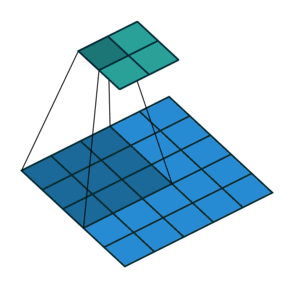
\includegraphics[width=4cm]{images/sconv}}
    {\centering Image from \href{https://github.com/vdumoulin/conv_arithmetic/blob/master/gif/no_padding_strides.gif}{github.com}}
\end{center}

\end{frame}


\begin{frame}
\frametitle{Convolutional Neural Networks}
\framesubtitle{Pooling}

How much pooling do we need?
\begin{itemize}
    \item Depends on task
    \item Usually $W_l$ and $H_l$ end up $<10$ %
\end{itemize}

\bigskip

Modern classification architectures pool down to $1\times1$ (!)
\begin{itemize}
    \item Via a final \emph{global average-pooling} layer
    \item Pooling using $\mean(\cdot)$ and $k=W_l=H_l$ %
\end{itemize}

\end{frame}


\begin{frame}
\frametitle{Convolutional Neural Networks}
\framesubtitle{Classification Backends}

Conv and pooling layers produce 3D tensors ($C_l\times W_l\times H_l$)

\bigskip

For classification we convert to vectors $\vx_l$
\begin{itemize}
    \item Flatten input tensor like we did earlier with images
\end{itemize}

\bigskip

Allows us to connect linear layers, resulting in
\begin{itemize}
    \item A linear or non-linear (MLP) classifier %
    \item That processes vectors of \emph{learned features} %
\end{itemize}

\end{frame}


\begin{frame}
\frametitle{Convolutional Neural Networks}
\framesubtitle{Classification Backends}

\begin{center}
    \copyrightbox[b]
    {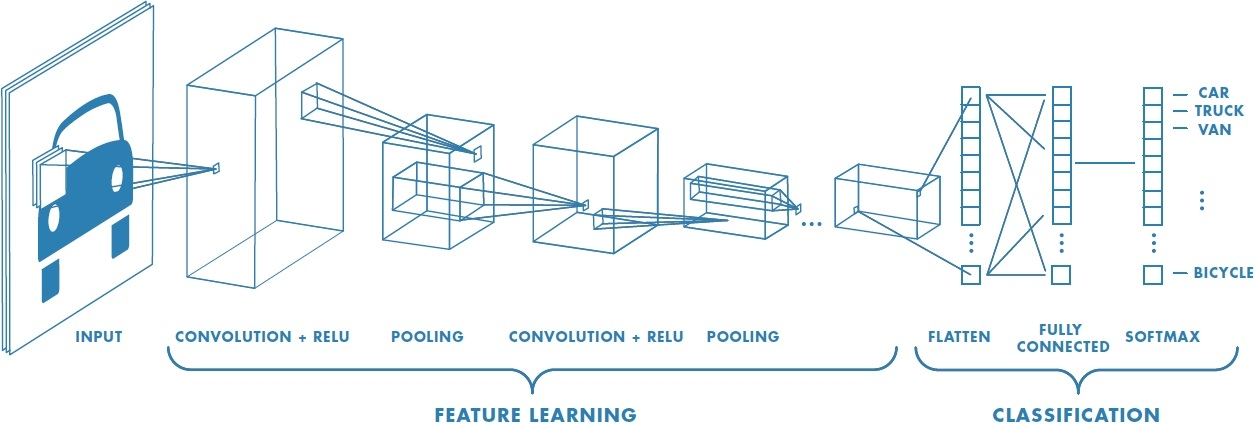
\includegraphics[width=10.5cm]{images/cnn}}
    {\centering Image from floydhub.com}
\end{center}

\end{frame}


\begin{frame}
\frametitle{Convolutional Neural Networks}
\framesubtitle{Classification Backends}

Modern architectures use linear classifiers
\begin{itemize}
    \item So the learned features are so powerful
    \item That the simplest classifier is sufficient (!)
\end{itemize}

\bigskip

We finally have task-specific high-level features %
\begin{itemize}
    \item Reason why deep learning is so powerful
\end{itemize}

\end{frame}


\begin{frame}
\frametitle{Convolutional Neural Networks}
\framesubtitle{CIFAR-10 Demo}

\begin{center}
    \copyrightbox[b]
    {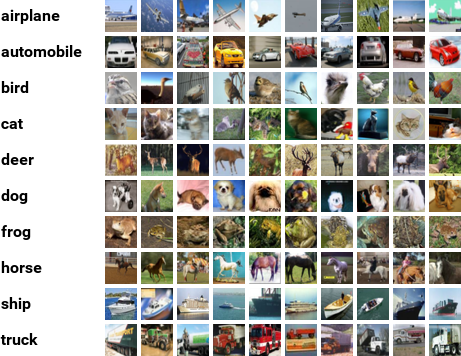
\includegraphics[width=6cm]{images/cifar10}}
    {\centering \href{https://cs.stanford.edu/people/karpathy/convnetjs/demo/cifar10.html}{Demo}}
\end{center}

\end{frame}


{
\setbeamertemplate{footline}{}
\begin{frame}

\begin{tikzpicture}[remember picture,overlay]
\fill[white] (current page.north west) rectangle (current page.south east);
\end{tikzpicture}

\begin{center}
\textcolor[rgb]{0.9,0.9,0.9}{blank page}
\end{center}

\end{frame}
}


\begin{frame}
\frametitle{Deep Image Classification}
\framesubtitle{Basic Classifier Design}

This concludes the basic layer types and purposes %
\begin{itemize}
    \item Conv + ReLU layers for feature extraction
    \item Pooling (or strided conv) layers for dimensionality reduction
    \item Linear layers for classification
\end{itemize}

\bigskip

The question is how to arrange these layers properly
\begin{itemize}
    \item Following slides introduce a simple recipe
    \item More advanced designs will covered in next lectures
\end{itemize}

\end{frame}


\begin{frame}
\frametitle{Deep Image Classification}
\framesubtitle{Basic Classifier Design}

Use square images, $H_0=W_0=R$ %
\begin{itemize}
    \item Resize images such that smaller side has size $R$
    \item Then extract a center crop of size $R\times R$
\end{itemize}

\bigskip

$R$ should be divisible by 2 many times
\begin{itemize}
    \item Avoid problems during pooling %
\end{itemize}

\end{frame}


\begin{frame}
\frametitle{Deep Image Classification}
\framesubtitle{Basic Classifier Design}

Start with small $R$ %
\begin{itemize}
    \item And test if increasing $R$ makes sense %
    \item $R=224$ is popular for classification %
    \item But much smaller $R$ might be sufficient %
\end{itemize}

\bigskip

Get $R$ below $100$ quickly via aggressive pooling %
\begin{itemize}
    \item To improve efficiency
    \item $R=224$: conv with $k=7,s=2$ $\Rightarrow$ $2\times2$ max-pooling %
\end{itemize}

\end{frame}


\begin{frame}
\frametitle{Deep Image Classification}
\framesubtitle{Basic Classifier Design}

Use conv $\Rightarrow$ conv $\Rightarrow$ pooling blocks
\begin{itemize}
    \item Conv layers with $k=3$, stride 1, padding, and ReLUs
    \item Pooling layers with $2\times2$ max-pooling with stride 2
\end{itemize}

\bigskip

Start with 32 or 64 feature maps %
\begin{itemize}
    \item Increase by factor 2 in each subsequent block
    \item Up to a maximum of 512 feature maps
\end{itemize}

\bigskip

Stack blocks until $R\leq7$
\begin{itemize}
    \item Usually means 4 or 5 such blocks %
\end{itemize}

\end{frame}


\begin{frame}
\frametitle{Deep Image Classification}
\framesubtitle{Basic Classifier Design}

Finish with linear classifier
\begin{itemize}
    \item Global average pooling
    \item Followed by linear layer with $T$ neurons
\end{itemize}

\bigskip

This recipe is a good starting point
\begin{itemize}
    \item Decent performance on many datasets (try yourself)
    \item Tune some hyperparameters depending on time budget
\end{itemize}

\end{frame}


\begin{frame}
\frametitle{Deep Image Classification}
\framesubtitle{Basic Classifier Design}

Example result with $R=224$

\bigskip

\begin{center}
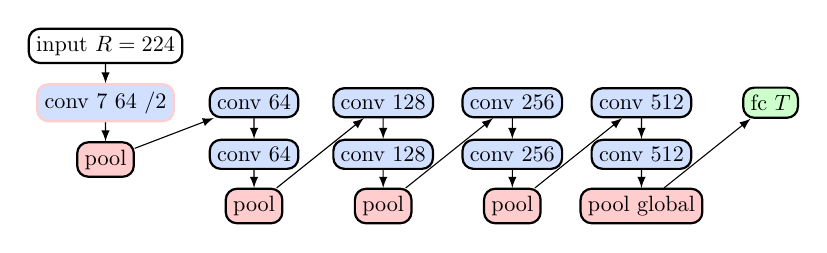
\begin{tikzpicture}[scale=0.82, every node/.style={scale=0.8}]
\def \n {0.8}
\def \s {2.0}
\node[draw, rectangle, rounded corners, thick] at (-0.3, 0.1*\n) (in) {input $R=224$};
\node[draw=xred, rectangle, rounded corners, thick, fill=xblue] at (-0.3, -1*\n) (conv1) {conv $7$ $64$ $/2$};
\node[draw, rectangle, rounded corners, thick, fill=xred] at (-0.3, -2.1*\n) (pool1) {pool};
\begin{scope}[on background layer]
\draw[->, >=latex] (in) -- (conv1);
\draw[->, >=latex] (conv1) -- (pool1);
\end{scope}
\node[draw, rectangle, rounded corners, thick, fill=xblue] at (\s, -1*\n) (conv3) {conv $64$};
\node[draw, rectangle, rounded corners, thick, fill=xblue] at (\s, -2*\n) (conv4) {conv $64$};
\node[draw, rectangle, rounded corners, thick, fill=xred] at (\s, -3*\n) (pool2) {pool};
\begin{scope}[on background layer]
\draw[->, >=latex] (pool1) -- (conv3);
\draw[->, >=latex] (conv3) -- (conv4);
\draw[->, >=latex] (conv4) -- (pool2);
\end{scope}
\node[draw, rectangle, rounded corners, thick, fill=xblue] at (2*\s, -1*\n) (conv5) {conv $128$};
\node[draw, rectangle, rounded corners, thick, fill=xblue] at (2*\s, -2*\n) (conv6) {conv $128$};
\node[draw, rectangle, rounded corners, thick, fill=xred] at (2*\s, -3*\n) (pool3) {pool};
\begin{scope}[on background layer]
\draw[->, >=latex] (pool2) -- (conv5);
\draw[->, >=latex] (conv5) -- (conv6);
\draw[->, >=latex] (conv6) -- (pool3);
\end{scope}
\node[draw, rectangle, rounded corners, thick, fill=xblue] at (3*\s, -1*\n) (conv8) {conv $256$};
\node[draw, rectangle, rounded corners, thick, fill=xblue] at (3*\s, -2*\n) (conv9) {conv $256$};
\node[draw, rectangle, rounded corners, thick, fill=xred] at (3*\s, -3*\n) (pool4) {pool};
\begin{scope}[on background layer]
\draw[->, >=latex] (pool3) -- (conv8);
\draw[->, >=latex] (conv8) -- (conv9);
\draw[->, >=latex] (conv9) -- (pool4);
\end{scope}
\node[draw, rectangle, rounded corners, thick, fill=xblue] at (4*\s, -1*\n) (conv11) {conv $512$};
\node[draw, rectangle, rounded corners, thick, fill=xblue] at (4*\s, -2*\n) (conv12) {conv $512$};
\node[draw, rectangle, rounded corners, thick, fill=xred] at (4*\s, -3*\n) (pool5) {pool global};
\begin{scope}[on background layer]
\draw[->, >=latex] (pool4) -- (conv11);
\draw[->, >=latex] (conv11) -- (conv12);
\draw[->, >=latex] (conv12) -- (pool5);
\end{scope}
\node[draw, rectangle, rounded corners, thick, fill=xgreen] at (5*\s, -1*\n) (fc1) {fc $T$};
\begin{scope}[on background layer]
\draw[->, >=latex] (pool5) -- (fc1);
\end{scope}
\end{tikzpicture}
\end{center}

\end{frame}


\begin{frame}
\frametitle{Deep Image Classification}
\framesubtitle{Basic Classifier Design}

Example result for for our cat vs.~dog problem ($R=32$)
\begin{itemize}
    \item Try different variants yourselves
\end{itemize}

\bigskip

\begin{center}
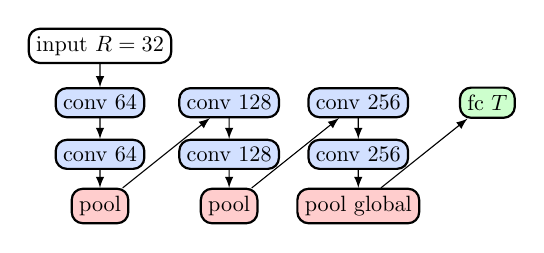
\begin{tikzpicture}[scale=0.82, every node/.style={scale=0.8}]
\def \n {0.8}
\def \s {2.0}
\node[draw, rectangle, rounded corners, thick] at (\s, 0.1*\n) (in) {input $R=32$};
\node[draw, rectangle, rounded corners, thick, fill=xblue] at (\s, -1*\n) (conv3) {conv $64$};
\node[draw, rectangle, rounded corners, thick, fill=xblue] at (\s, -2*\n) (conv4) {conv $64$};
\node[draw, rectangle, rounded corners, thick, fill=xred] at (\s, -3*\n) (pool2) {pool};
\begin{scope}[on background layer]
\draw[->, >=latex] (in) -- (conv3);
\draw[->, >=latex] (conv3) -- (conv4);
\draw[->, >=latex] (conv4) -- (pool2);
\end{scope}
\node[draw, rectangle, rounded corners, thick, fill=xblue] at (2*\s, -1*\n) (conv5) {conv $128$};
\node[draw, rectangle, rounded corners, thick, fill=xblue] at (2*\s, -2*\n) (conv6) {conv $128$};
\node[draw, rectangle, rounded corners, thick, fill=xred] at (2*\s, -3*\n) (pool3) {pool};
\begin{scope}[on background layer]
\draw[->, >=latex] (pool2) -- (conv5);
\draw[->, >=latex] (conv5) -- (conv6);
\draw[->, >=latex] (conv6) -- (pool3);
\end{scope}
\node[draw, rectangle, rounded corners, thick, fill=xblue] at (3*\s, -1*\n) (conv8) {conv $256$};
\node[draw, rectangle, rounded corners, thick, fill=xblue] at (3*\s, -2*\n) (conv9) {conv $256$};
\node[draw, rectangle, rounded corners, thick, fill=xred] at (3*\s, -3*\n) (pool4) {pool global};
\begin{scope}[on background layer]
\draw[->, >=latex] (pool3) -- (conv8);
\draw[->, >=latex] (conv8) -- (conv9);
\draw[->, >=latex] (conv9) -- (pool4);
\end{scope}
\node[draw, rectangle, rounded corners, thick, fill=xgreen] at (4*\s, -1*\n) (fc1) {fc $T$};
\begin{scope}[on background layer]
\draw[->, >=latex] (pool4) -- (fc1);
\end{scope}
\end{tikzpicture}
\end{center}

\end{frame}


\begin{frame}[fragile]
\frametitle{Deep Image Classification}
\framesubtitle{PyTorch Implementation}

Let's implement the above network in PyTorch
\begin{itemize}
    \item Based on subnetworks for components
    \item One of many options (could just stack layers)
\end{itemize}

\bigskip

First import the required modules:

\medskip

\footnotesize
\begin{verbatim}
import torch
import torch.nn as nn
\end{verbatim}

\end{frame}


\begin{frame}[fragile]
\frametitle{Deep Image Classification}
\framesubtitle{PyTorch Implementation}

Networks always process samples in batches
\begin{itemize}
    \item So input tensor is 4D
    \item Batch size is 1 for single images
\end{itemize}

\medskip

\footnotesize
\begin{verbatim}
x = torch.zeros(  # dummy input
  4,     # batch size
  3,     # number of input channels
  224,   # imput height
  224    # input width
)
\end{verbatim}

\end{frame}


\begin{frame}[fragile]
\frametitle{Deep Image Classification}
\framesubtitle{PyTorch Implementation}

Frontend first

\medskip

\footnotesize
\begin{verbatim}
def frontend(nin, nout):
  return nn.Sequential(
    nn.Conv2d(nin, nout, kernel_size=7, padding=3, stride=2),
    nn.ReLU(inplace=True),
    nn.MaxPool2d(kernel_size=2, stride=2)
  )

f = frontend(3, 64)
y = f(x)  # size of y is [4, 64, 56, 56]
\end{verbatim}

\end{frame}


\begin{frame}[fragile]
\frametitle{Deep Image Classification}
\framesubtitle{PyTorch Implementation}

Basic building blocks

\medskip

\footnotesize
\begin{verbatim}
def conv3(nin, nout):
  return nn.Sequential(
    nn.Conv2d(nin, nout, kernel_size=3, padding=1),
    nn.ReLU(inplace=True)
  )

def block(nin, nout=None, pool=True):
  nout = nout if nout else nin * 2
  return nn.Sequential(
    conv3(nin, nout),
    conv3(nout, nout),
    nn.MaxPool2d(kernel_size=2, stride=2) if pool else nn.Identity()
  )
\end{verbatim}

\end{frame}


\begin{frame}[fragile]
\frametitle{Deep Image Classification}
\framesubtitle{PyTorch Implementation}

Complete network

\medskip

\footnotesize
\begin{verbatim}
net = nn.Sequential(
  frontend(3, 64),
  block(64, 64),
  block(64),
  block(128),
  block(256, pool=False),
  nn.AvgPool2d(kernel_size=7),
  nn.Flatten(),
  nn.Linear(512, 10)  # assuming 10 classes
)

y = net(x)  # size of y is [4, 10]
\end{verbatim}

\end{frame}


\renewcommand\emph[1]{\oldemph{#1}}

\begin{frame}
\frametitle{Bibliography}

[1] Goodfellow et al. Deep Learning. 2016.

\end{frame}


\end{document}
